\documentclass[border=4pt]{standalone}
\usepackage{fontspec}
\IfFileExists{../fonts/times.ttf}{
  \setmainfont{times.ttf}[
    Path           = ../fonts/,
    BoldFont       = timesbd.ttf,
    ItalicFont     = timesi.ttf,
    BoldItalicFont = timesbi.ttf
  ]
}{\usepackage{mathptmx}}
\usepackage{tikz}
\usetikzlibrary{arrows.meta,positioning,calc}
\begin{document}
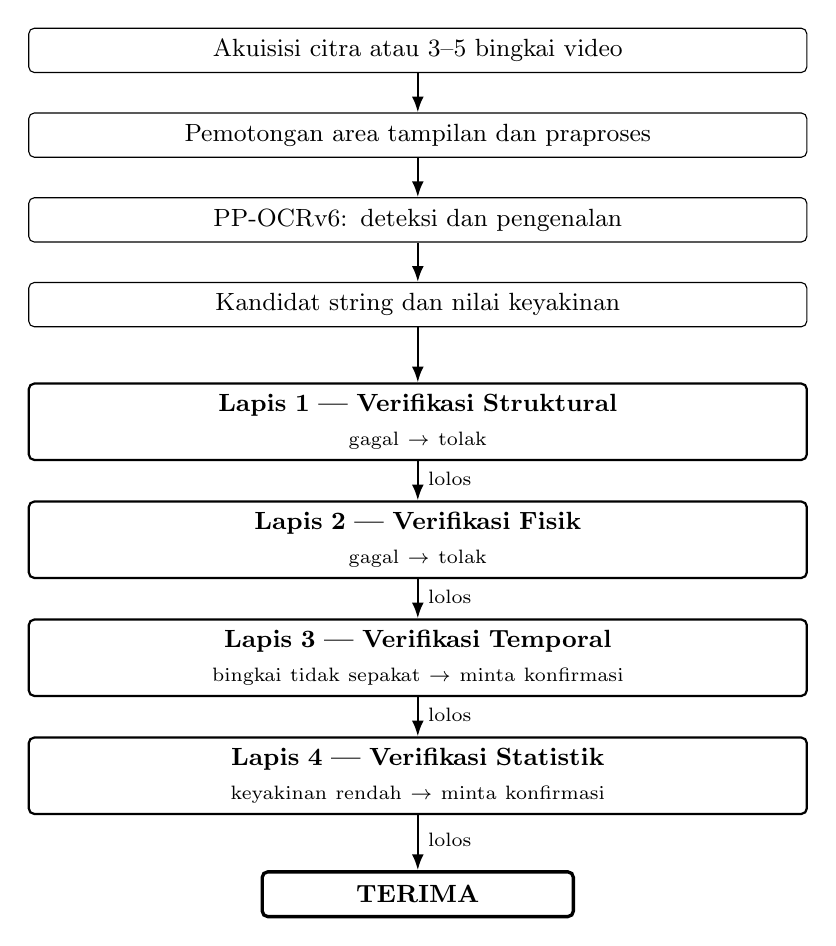
\begin{tikzpicture}[
  node distance=0.5cm,
  kotak/.style={rectangle, draw, rounded corners=2pt, align=center,
                text width=9.6cm, inner sep=4pt, font=\small},
  lapis/.style={rectangle, draw, thick, rounded corners=2pt, align=center,
                text width=9.6cm, inner sep=4pt, font=\small},
  akhir/.style={rectangle, draw, very thick, rounded corners=2pt,
                align=center, text width=3.6cm, inner sep=5pt, font=\small},
  panah/.style={-{Latex[length=2mm]}, thick}
]
\node[kotak] (aku) {Akuisisi citra atau 3--5 bingkai video};
\node[kotak, below=of aku] (pra) {Pemotongan area tampilan dan praproses};
\node[kotak, below=of pra] (ocr) {PP-OCRv6: deteksi dan pengenalan};
\node[kotak, below=of ocr] (kan) {Kandidat string dan nilai keyakinan};

\node[lapis, below=0.7cm of kan] (l1)
  {\textbf{Lapis 1 --- Verifikasi Struktural}\\[1pt]
   {\scriptsize gagal $\rightarrow$ tolak}};
\node[lapis, below=of l1] (l2)
  {\textbf{Lapis 2 --- Verifikasi Fisik}\\[1pt]
   {\scriptsize gagal $\rightarrow$ tolak}};
\node[lapis, below=of l2] (l3)
  {\textbf{Lapis 3 --- Verifikasi Temporal}\\[1pt]
   {\scriptsize bingkai tidak sepakat $\rightarrow$ minta konfirmasi}};
\node[lapis, below=of l3] (l4)
  {\textbf{Lapis 4 --- Verifikasi Statistik}\\[1pt]
   {\scriptsize keyakinan rendah $\rightarrow$ minta konfirmasi}};

\node[akhir, below=0.7cm of l4] (terima) {\textbf{TERIMA}};

\draw[panah] (aku) -- (pra);
\draw[panah] (pra) -- (ocr);
\draw[panah] (ocr) -- (kan);
\draw[panah] (kan) -- (l1);
\draw[panah] (l1) -- node[right, font=\scriptsize, pos=0.45] {lolos} (l2);
\draw[panah] (l2) -- node[right, font=\scriptsize, pos=0.45] {lolos} (l3);
\draw[panah] (l3) -- node[right, font=\scriptsize, pos=0.45] {lolos} (l4);
\draw[panah] (l4) -- node[right, font=\scriptsize, pos=0.45] {lolos} (terima);
\end{tikzpicture}
\end{document}
